% ============================================================
%  Semaine 1 — Fondamentaux du web & environnement
%  Polycopié étudiant — cfpt·i | Anne Terrier
%  Charte graphique : charte cfpt·i originale, police sans-serif
% ============================================================
\documentclass[a4paper,11pt]{article}

\usepackage[T1]{fontenc}
\usepackage[utf8]{inputenc}
\usepackage[scaled=0.92]{helvet}
\renewcommand{\familydefault}{\sfdefault}
\usepackage[top=2.5cm, bottom=2.5cm, left=2.5cm, right=2.5cm, headheight=40pt]{geometry}
\usepackage{microtype}

\usepackage[dvipsnames,svgnames,table]{xcolor}
\usepackage{graphicx}
\usepackage{tikz}
\usetikzlibrary{positioning, shapes.geometric, arrows.meta, fit, backgrounds, decorations.pathreplacing}
\usepackage{booktabs}
\usepackage{tabularx}
\usepackage{array}
\usepackage{enumitem}
\usepackage[most]{tcolorbox}
\usepackage{fancyhdr}
\usepackage{lastpage}
\usepackage{titlesec}
\usepackage{listings}
\usepackage[hidelinks]{hyperref}

% ---------------------------------------------------------------
% Palette cfpt·i originale
% ---------------------------------------------------------------
\definecolor{cfptYellow}{HTML}{F5C400}
\definecolor{cfptBlack}{HTML}{1A1A1A}
\definecolor{cfptDarkGrey}{HTML}{555555}
\definecolor{cfptGrey}{HTML}{F2F2F2}
\definecolor{accentBlue}{HTML}{1D4E89}
\definecolor{lightBlue}{HTML}{D6E4F0}
\definecolor{codeGrey}{HTML}{F5F5F5}
\definecolor{successGreen}{HTML}{1E7145}
\definecolor{warningOrange}{HTML}{C55A11}

% Alias (le contenu du document utilise ces noms) vers la palette ci-dessus
\colorlet{uniInk}{cfptBlack}
\colorlet{uniNavy}{accentBlue}
\colorlet{uniTeal}{successGreen}
\colorlet{uniGold}{warningOrange}
\colorlet{uniGrey}{cfptDarkGrey}
\colorlet{uniPaper}{cfptGrey}
\colorlet{uniRule}{cfptDarkGrey!35}

\color{cfptBlack}

% --- En-tête / pied de page ---
\pagestyle{fancy}
\fancyhf{}
\renewcommand{\headrulewidth}{0pt}
\fancyhead[L]{\IfFileExists{Semaine1/images/cfpti.png}{
\includegraphics[height=18pt]{Semaine1/images/cfpti.png}}{}}
\fancyhead[C]{\color{cfptDarkGrey}\small\textit{Développement Web --- Classe passerelle}}
\fancyhead[R]{\color{cfptDarkGrey}\small\textit{Semaine 1}}
\fancyfoot[L]{\color{cfptDarkGrey}\footnotesize Anne Terrier}
\fancyfoot[C]{\color{cfptDarkGrey}\footnotesize {Fondamentaux du web \& environnement}}
\fancyfoot[R]{\color{cfptDarkGrey}\footnotesize Page \thepage\ sur \pageref{LastPage}}
\renewcommand{\footrulewidth}{0.4pt}

% --- Titres sections : bandeau plein largeur ---
\newcommand{\sectionbox}[1]{%
  \colorbox{accentBlue}{%
    \parbox[c][1.6em][c]{\dimexpr\linewidth-2\fboxsep\relax}{%
      \color{white}\large\bfseries\hspace{4pt}\arabic{section}\qquad #1}}}

\newcommand{\sectionboxstar}[1]{%
  \colorbox{accentBlue}{%
    \parbox[c][1.6em][c]{\dimexpr\linewidth-2\fboxsep\relax}{%
      \color{white}\large\bfseries\hspace{4pt}#1}}}

\titleformat{\section}{\normalfont}{}{0pt}{\sectionbox}
\titleformat{name=\section,numberless}{\normalfont}{}{0pt}{\sectionboxstar}
\titleformat{\subsection}{\color{accentBlue}\normalsize\bfseries}{\rule[-.3ex]{3pt}{1.3em}}{6pt}{}
\titlespacing{\section}{0pt}{18pt}{8pt}
\titlespacing{\subsection}{0pt}{12pt}{4pt}

% --- supprime les retraits de paragraphe ---
\setlength{\parindent}{0pt}

% --- Listes ---
\setlist[itemize]{itemsep=3pt, topsep=4pt, parsep=0pt,
  leftmargin=1.4em, label={\color{cfptYellow}\textbullet}}
\setlist[itemize,2]{label={\color{cfptDarkGrey}--}, leftmargin=1.8em}
\setlist[enumerate]{itemsep=4pt, topsep=4pt, leftmargin=1.6em}

% --- Boîtes tcolorbox ---
\tcbset{
  definition/.style={
    colback=lightBlue!30, colframe=accentBlue,
    fonttitle=\bfseries\small\color{accentBlue},
    boxrule=0.8pt, arc=3pt,
    left=6pt, right=6pt, top=4pt, bottom=4pt,
    toptitle=2pt, bottomtitle=2pt},
  attention/.style={
    colback=cfptYellow!20, colframe=cfptYellow!80!black,
    fonttitle=\bfseries\small,
    boxrule=0.8pt, arc=3pt,
    left=6pt, right=6pt, top=4pt, bottom=4pt,
    toptitle=2pt, bottomtitle=2pt},
  astuce/.style={
    colback=successGreen!8, colframe=successGreen,
    fonttitle=\bfseries\small\color{successGreen},
    boxrule=0.8pt, arc=3pt,
    left=6pt, right=6pt, top=4pt, bottom=4pt,
    toptitle=2pt, bottomtitle=2pt},
  corrige/.style={
    colback=cfptGrey, colframe=cfptDarkGrey,
    fonttitle=\bfseries\small\color{cfptDarkGrey},
    boxrule=0.8pt, arc=3pt,
    left=6pt, right=6pt, top=4pt, bottom=4pt,
    toptitle=2pt, bottomtitle=2pt}
}

% --- Listings code ---
\lstset{
  basicstyle=\ttfamily\small,
  backgroundcolor=\color{codeGrey},
  frame=single, framerule=0.4pt,
  rulecolor=\color{cfptDarkGrey!40},
  breaklines=true,
  keywordstyle=\color{accentBlue}\bfseries,
  commentstyle=\color{cfptDarkGrey}\itshape,
  stringstyle=\color{successGreen},
  showstringspaces=false,
  numbers=left, numberstyle=\tiny\color{cfptDarkGrey},
  numbersep=8pt,
  captionpos=b,
}
\renewcommand{\lstlistingname}{Extrait}

\renewcommand{\arraystretch}{1.3}

% ============================================================
\begin{document}
% ============================================================

% --- Bandeau titre ---
\begin{tcolorbox}[
  colback=accentBlue, colframe=accentBlue,
  arc=4pt, left=12pt, right=12pt, top=10pt, bottom=10pt]
  \begin{minipage}{0.72\linewidth}
    {\color{white}\Large\bfseries Semaine 1}\\[4pt]
    {\color{white}\Large\bfseries Fondamentaux du web \& environnement}\\[4pt]
    {\color{lightBlue}\normalsize Anne Terrier --- Développement web, classe passerelle}
  \end{minipage}
  \hfill
  \begin{minipage}{0.22\linewidth}
    \raggedleft
    \begin{tabular}{rl}
      \multicolumn{2}{r}{\color{white}\small \today} \\
      \color{lightBlue}\small Cours & \color{white}\small 4h \\
      \color{lightBlue}\small TP    & \color{white}\small 4h \\
    \end{tabular}
  \end{minipage}
\end{tcolorbox}

\vspace{6pt}
\begin{tcolorbox}[definition, title={Objectifs de la semaine}]
\begin{itemize}
  \item Comprendre le modèle client/serveur et le fonctionnement du web
  \item Distinguer les rôles de HTML, CSS et JavaScript
  \item Distinguer un site statique d'un site dynamique
  \item Installer et configurer son environnement de développement
  \item Créer son premier dépôt Git et effectuer un premier commit
\end{itemize}
\end{tcolorbox}

% ============================================================
\section{Comment fonctionne le web ?}
% ============================================================

Quand tu tapes \texttt{https://www.hepia.ch} dans ton navigateur, une série d'échanges invisibles se produit en quelques millisecondes. Comprendre ce mécanisme est le point de départ de tout développeur web.

\subsection{Le modèle client / serveur}

\begin{figure}[h]
    \centering
    
\includegraphics[width=1\textwidth]{Semaine1/images/client serveur.jpg}
    \caption{Architecteur Client-Serveur}
    \label{fig:ClientServeur}
\end{figure}




\begin{tcolorbox}[definition, title={Définition --- Client et serveur}]
\textbf{Client} : programme qui \textit{demande} une ressource (le navigateur).\\
\textbf{Serveur} : programme qui \textit{répond} à la demande en envoyant des fichiers ou des données.\\
La communication se fait via le protocole \textbf{HTTP} (ou \textbf{HTTPS} pour la version sécurisée).
\end{tcolorbox}

\subsection{Anatomie d'une URL}

\vspace{8pt}
\begin{center}
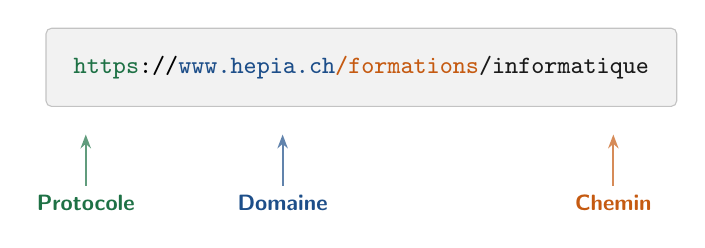
\begin{tikzpicture}[font=\small]
  \node[fill=uniPaper, draw=uniRule, thin, rounded corners=2pt,
        inner sep=10pt] (url)
  {\texttt{%
    \textcolor{uniTeal}{https}://%
    \textcolor{uniNavy}{www.hepia.ch}%
    \textcolor{uniGold}{/formations}%
    \textcolor{uniInk}{/informatique}}};

  \node[below=1cm of url, xshift=-3.5cm,
        text=uniTeal, font=\footnotesize\bfseries] (lp) {Protocole};
  \node[below=1cm of url, xshift=-1.0cm,
        text=uniNavy, font=\footnotesize\bfseries] (ld) {Domaine};
  \node[below=1cm of url, xshift=3.2cm,
        text=uniGold, font=\footnotesize\bfseries] (lc) {Chemin};

  \draw[-{Stealth[length=5pt]}, uniTeal!70, thick] (lp.north) -- ++(0,0.65);
  \draw[-{Stealth[length=5pt]}, uniNavy!70, thick]   (ld.north) -- ++(0,0.65);
  \draw[-{Stealth[length=5pt]}, uniGold!70, thick] (lc.north) -- ++(0,0.65);
\end{tikzpicture}
\end{center}

\subsection{DNS --- de l'adresse au nom}

Un ordinateur ne comprend pas \texttt{www.hepia.ch} : il a besoin d'une adresse numérique, appelée \textbf{adresse IP} (par exemple \texttt{192.0.2.34}). Le \textbf{DNS} (\textit{Domain Name System}) est le service qui traduit un nom de domaine lisible en adresse IP.

\begin{tcolorbox}[astuce, title={Analogie --- L'annuaire téléphonique}]
Le DNS fonctionne comme un annuaire : tu connais le \textit{nom} d'une personne (le domaine), l'annuaire te donne son \textit{numéro} (l'adresse IP), et c'est ce numéro qui permet réellement d'établir la communication.
\end{tcolorbox}

\vspace{2pt}
\noindent\textbf{Étapes simplifiées :}
\begin{enumerate}
  \item Le navigateur demande au DNS : « quelle est l'adresse IP de \texttt{www.hepia.ch} ? »
  \item Le serveur DNS répond avec l'adresse IP correspondante
  \item Le navigateur peut alors envoyer sa requête HTTP directement à cette adresse
\end{enumerate}

\subsection{Les codes de statut HTTP}

\begin{center}
\begin{tabularx}{0.85\linewidth}{ccX}
  \toprule
  \rowcolor{uniNavy}
  \color{white}\textbf{Code} &
  \color{white}\textbf{Signification} &
  \color{white}\textbf{Quand ?} \\
  \midrule
  \rowcolor{uniPaper}
  \texttt{200} & OK & Tout s'est bien passé \\
  \texttt{301} & Redirection & La page a changé d'adresse \\
  \rowcolor{uniPaper}
  \texttt{404} & Not Found & La page n'existe pas \\
  \texttt{500} & Server Error & Erreur côté serveur \\
  \bottomrule
\end{tabularx}
\end{center}

\subsection{Sites statiques et sites dynamiques}

\begin{tcolorbox}[definition, title={Définition --- Statique vs dynamique}]
Un \textbf{site statique} renvoie toujours le même contenu au client : le fichier HTML existe déjà sur le serveur et est envoyé tel quel.\\
Un \textbf{site dynamique} génère le contenu à la demande, souvent à partir d'une base de données : deux visiteurs, ou deux moments différents, peuvent recevoir des pages différentes.
\end{tcolorbox}

\begin{center}
\begin{tabularx}{\linewidth}{lXX}
  \toprule
  \rowcolor{uniNavy}
  \color{white}\textbf{} &
  \color{white}\textbf{Site statique} &
  \color{white}\textbf{Site dynamique} \\
  \midrule
  \rowcolor{uniPaper}
  Contenu & Identique pour tout le monde & Généré à chaque requête \\
  Exemple & Page vitrine simple, portfolio & Forum, boutique en ligne, réseau social \\
  \rowcolor{uniPaper}
  Techniquement & Fichiers HTML/CSS/JS seuls & Serveur applicatif (Node.js) + base de données \\
\end{tabularx}
\end{center}

\begin{tcolorbox}[attention, title={Où se situe MiniForum ?}]
Le projet fil rouge \textbf{MiniForum} commence comme un site \textbf{statique} (données codées en dur en semaine 1--5), puis devient \textbf{dynamique} à partir de la phase 3, lorsqu'il se connecte à une vraie base de données via Node.js/Express.
\end{tcolorbox}

% ============================================================
\section{Les trois langages côté clients}
% ============================================================

\vspace{6pt}
\begin{center}
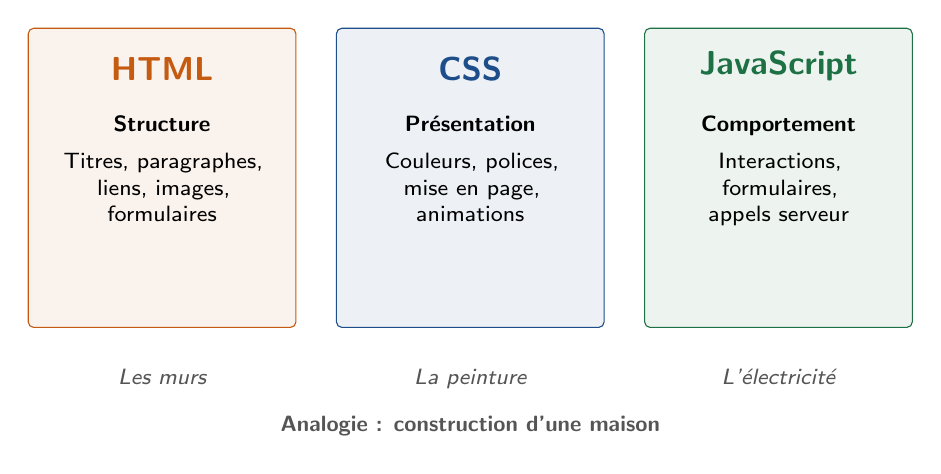
\begin{tikzpicture}[font=\small]

\node[draw=uniGold, thin, rounded corners=2pt, fill=uniGold!8,
      minimum width=3.4cm, minimum height=3.8cm, align=center] (html) at (0,0) {};
\node[font=\bfseries\large, text=uniGold, above=-0.8cm of html] {HTML};
\node[below=1cm of html.north, align=center, text width=3cm, font=\footnotesize]
  {\textbf{Structure}\\[4pt] Titres, paragraphes,\\liens, images,\\formulaires};

\node[draw=uniNavy, thin, rounded corners=2pt, fill=uniNavy!8,
      minimum width=3.4cm, minimum height=3.8cm, align=center,
      right=0.5cm of html] (css) {};
\node[font=\bfseries\large, text=uniNavy, above=-0.8cm of css] {CSS};
\node[below=1cm of css.north, align=center, text width=3cm, font=\footnotesize]
  {\textbf{Présentation}\\[4pt] Couleurs, polices,\\mise en page,\\animations};

\node[draw=uniTeal, thin, rounded corners=2pt, fill=uniTeal!8,
      minimum width=3.4cm, minimum height=3.8cm, align=center,
      right=0.5cm of css] (js) {};
\node[font=\bfseries\large, text=uniTeal, above=-0.8cm of js] {JavaScript};
\node[below=1cm of js.north, align=center, text width=3cm, font=\footnotesize]
  {\textbf{Comportement}\\[4pt] Interactions,\\formulaires,\\appels serveur};

\node[below=0.4cm of html.south, font=\footnotesize\itshape, text=uniGrey]
  {Les murs};
\node[below=0.4cm of css.south, font=\footnotesize\itshape, text=uniGrey]
  {La peinture};
\node[below=0.4cm of js.south, font=\footnotesize\itshape, text=uniGrey]
  {L'électricité};

\node[below=1cm of css.south, font=\footnotesize\bfseries, text=uniGrey]
  {Analogie : construction d'une maison};
\end{tikzpicture}
\end{center}
\vspace{6pt}

\begin{tcolorbox}[attention, title={Important --- Qui exécute quoi ?}]
\textbf{HTML, CSS et JavaScript} s'exécutent dans le \textbf{navigateur} (côté client).
\end{tcolorbox}

\subsection{Un premier exemple}

\begin{lstlisting}[language=HTML, caption={index.html --- Structure}]
<!DOCTYPE html>
<html lang="fr">
<head>
  <meta charset="UTF-8">
  <title>MiniForum</title>
  <link rel="stylesheet" href="style.css">
</head>
<body>
  <h1>Bienvenue sur MiniForum</h1>
  <button id="btn">Cliquez-moi</button>
  <script src="app.js"></script>
</body>
</html>
\end{lstlisting}

\begin{lstlisting}[language=HTML, caption={style.css --- Présentation}]
button {
  background-color: #1D3557; /* bleu marine */
  color: white;
  padding: 10px 20px;
  border: none;
  border-radius: 4px;
  cursor: pointer;
}
\end{lstlisting}

\begin{lstlisting}[language=bash, caption={app.js --- Comportement}]
const btn = document.getElementById('btn');
btn.addEventListener('click', () => {
  alert('Bonjour depuis JavaScript !');
});
\end{lstlisting}

% ============================================================
\section{Les langages côté serveur}
% ============================================================
Jusqu'à présent, nous avons vu les langages exécutés dans le navigateur :
\textbf{HTML}, \textbf{CSS} et \textbf{JavaScript}. Mais une application web doit souvent enregistrer et récupérer des données.
Pour cela, le navigateur communique avec un programme exécuté sur un serveur.

\begin{tcolorbox}[definition, title={Définition --- Langage côté serveur}]
Un langage côté serveur est exécuté sur le serveur.
Il reçoit une requête du navigateur, traite cette requête et renvoie une réponse.
\end{tcolorbox}

\subsection{Client et serveur}

Le fonctionnement peut être résumé ainsi :

\begin{center}
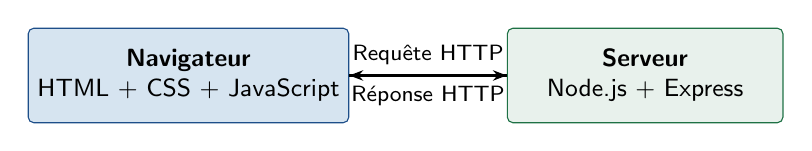
\begin{tikzpicture}[font=\small]

\node[
  draw=accentBlue,
  fill=lightBlue,
  rounded corners=2pt,
  minimum width=3.5cm,
  minimum height=1.2cm,
  align=center
] (client)
{\textbf{Navigateur}\\
HTML + CSS + JavaScript};

\node[
  draw=successGreen,
  fill=successGreen!10,
  rounded corners=2pt,
  minimum width=3.5cm,
  minimum height=1.2cm,
  align=center,
  right=2cm of client
] (server)
{\textbf{Serveur}\\
Node.js + Express};

\draw[-{Stealth[length=5pt]}, thick]
(client) -- node[above, font=\footnotesize]{Requête HTTP} (server);

\draw[-{Stealth[length=5pt]}, thick]
(server) -- node[below, font=\footnotesize]{Réponse HTTP} (client);

\end{tikzpicture}
\end{center}

Le serveur peut également communiquer avec une base de données :

\begin{center}
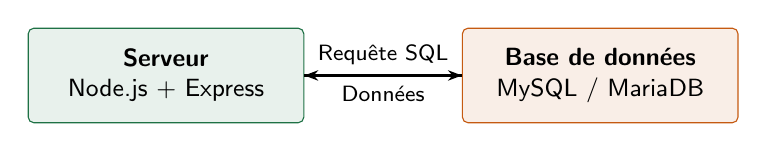
\begin{tikzpicture}[font=\small]

\node[
  draw=successGreen,
  fill=successGreen!10,
  rounded corners=2pt,
  minimum width=3.5cm,
  minimum height=1.2cm,
  align=center
] (server)
{\textbf{Serveur}\\
Node.js + Express};

\node[
  draw=warningOrange,
  fill=warningOrange!10,
  rounded corners=2pt,
  minimum width=3.5cm,
  minimum height=1.2cm,
  align=center,
  right=2cm of server
] (database)
{\textbf{Base de données}\\
MySQL / MariaDB};

\draw[-{Stealth[length=5pt]}, thick]
(server) -- node[above, font=\footnotesize]{Requête SQL} (database);

\draw[-{Stealth[length=5pt]}, thick]
(database) -- node[below, font=\footnotesize]{Données} (server);

\end{tikzpicture}
\end{center}

\subsection{Quelques langages côté serveur}

Il existe de nombreux langages permettant de développer des applications web.

\begin{center}
\renewcommand{\arraystretch}{1.0}
\begin{tabularx}{\linewidth}{p{4cm}X}
\toprule
\rowcolor{uniNavy}
\color{white}\textbf{Langage} &
\color{white}\textbf{Exemple d'utilisation}\\
\midrule
\rowcolor{uniPaper}
PHP & Sites et applications web\\
Python & Applications web et API\\
Java & Applications d'entreprise\\
C\# & Applications web avec ASP.NET\\
\rowcolor{uniPaper}
JavaScript avec Node.js & Serveurs web et API\\
\bottomrule
\end{tabularx}
\end{center}

\subsection{Node.js}

Dans ce cours, nous utiliserons \textbf{Node.js}.

Node.js permet d'exécuter du JavaScript en dehors du navigateur.

Il permet notamment de :

\begin{itemize}
  \item créer un serveur web ;
  \item recevoir des requêtes HTTP ;
  \item communiquer avec une base de données ;
  \item créer des API.
\end{itemize}

\begin{tcolorbox}[attention, title={Important --- Côté client et côté serveur}]
\textbf{JavaScript côté client} s'exécute dans le navigateur.

\textbf{JavaScript côté serveur} s'exécute sur le serveur avec Node.js.
\end{tcolorbox}

% ============================================================
\section{La stack du cours}
% ============================================================

Dans notre projet \textbf{MiniForum}, les différentes technologies auront les rôles suivants :

\vspace{8pt}
\begin{center}
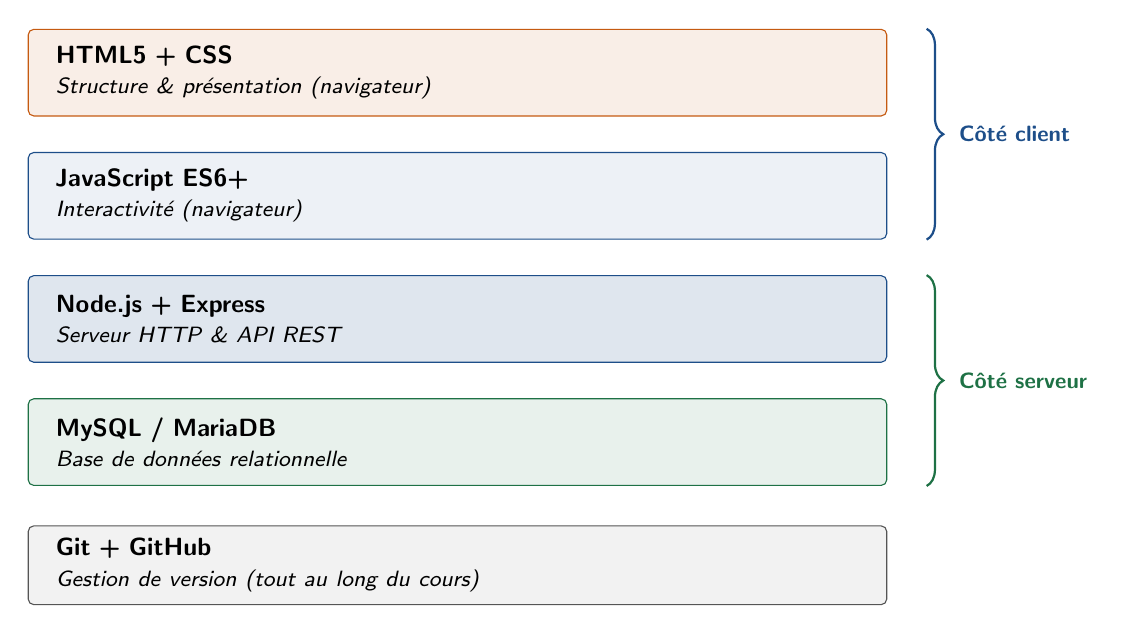
\begin{tikzpicture}[font=\small, node distance=0.45cm,
  layer/.style={draw=uniGrey, thin, rounded corners=2pt, text width=10.2cm,
    minimum height=1.1cm, align=left, inner xsep=10pt}]

\node[layer, fill=uniGold!10, draw=uniGold] (html)
  {\textbf{HTML5 + CSS}\\\footnotesize\textit{Structure \& présentation (navigateur)}};

\node[layer, fill=uniNavy!8, draw=uniNavy, below=of html] (js)
  {\textbf{JavaScript ES6+}\\\footnotesize\textit{Interactivité (navigateur)}};

\node[layer, fill=uniNavy!14, draw=uniNavy, below=of js] (node)
  {\textbf{Node.js + Express}\\\footnotesize\textit{Serveur HTTP \& API REST}};

\node[layer, fill=uniTeal!10, draw=uniTeal, below=of node] (sql)
  {\textbf{MySQL / MariaDB}\\\footnotesize\textit{Base de données relationnelle}};

\draw[decorate, decoration={brace,amplitude=6pt}, uniNavy, thick]
  ([xshift=0.5cm]html.north east) -- ([xshift=0.5cm]js.south east)
  node[midway, right=8pt, font=\footnotesize\bfseries, text=uniNavy]{Côté client};

\draw[decorate, decoration={brace,amplitude=6pt}, uniTeal, thick]
  ([xshift=0.5cm]node.north east) -- ([xshift=0.5cm]sql.south east)
  node[midway, right=8pt, font=\footnotesize\bfseries, text=uniTeal]{Côté serveur};

\node[layer, fill=uniPaper, draw=uniGrey,
      minimum height=1.0cm, below=0.5cm of sql] (git)
  {\textbf{Git + GitHub}\\\footnotesize\textit{Gestion de version (tout au long du cours)}};

\end{tikzpicture}
\end{center}

\begin{tcolorbox}[astuce, title={A retenir}]
Une application web complète est généralement composée de trois parties :

\begin{itemize}
  \item une interface côté client ;
  \item un serveur côté serveur ;
  \item une base de données.
\end{itemize}

Dans ce cours, nous utiliserons JavaScript des deux côtés :
\textbf{JavaScript dans le navigateur} et
\textbf{Node.js sur le serveur}.
\end{tcolorbox}

% ============================================================
\section{Environnement de développement}
% ============================================================

\subsection{Outils à installer}

\begin{tcolorbox}[definition, title={Liste des outils --- Semaine 1}]
\begin{itemize}
  \item \textbf{Visual Studio Code} \hfill \texttt{code.visualstudio.com}
  \item \textbf{Node.js LTS (v20+)} \hfill \texttt{nodejs.org}
  \item \textbf{Git} \hfill \texttt{git-scm.com}
  \item \textbf{Compte GitHub} \hfill \texttt{github.com}
\end{itemize}
\end{tcolorbox}

\subsection{Extensions VS Code recommandées}

\begin{center}
\renewcommand{\arraystretch}{1.0}
\begin{tabularx}{\linewidth}{p{4cm}X}
  \toprule
  \rowcolor{uniNavy}
  \color{white}\textbf{Extension} & \color{white}\textbf{Utilité} \\
  \midrule
  \rowcolor{uniPaper}
  Prettier      & Formatage automatique du code \\
  ESLint        & Détection d'erreurs JavaScript \\
  \rowcolor{uniPaper}
  Live Server   & Rechargement automatique du navigateur \\
  REST Client   & Tester les routes API depuis VS Code \\
  \rowcolor{uniPaper}
  GitLens       & Visualiser l'historique Git dans l'éditeur \\
  \bottomrule
\end{tabularx}
\end{center}

\subsection{Premiers pas dans le terminal}

Git et Node.js s'utilisent en ligne de commande. Quelques commandes suffisent pour naviguer dans les dossiers de ton projet.

\begin{center}
\renewcommand{\arraystretch}{1.0}
\begin{tabularx}{\linewidth}{p{4cm}X}
  \toprule
  \rowcolor{uniNavy}
  \color{white}\textbf{Commande} & \color{white}\textbf{Effet} \\
  \midrule
  \rowcolor{uniPaper}
  \texttt{pwd}        & Affiche le dossier courant \\
  \texttt{ls} (ou \texttt{dir})  & Liste le contenu du dossier courant \\
  \rowcolor{uniPaper}
  \texttt{cd nom-dossier} & Se déplace dans un sous-dossier \\
  \texttt{cd ..}      & Remonte d'un niveau \\
  \rowcolor{uniPaper}
  \texttt{mkdir nom}  & Crée un nouveau dossier \\
  \texttt{touch nom.txt} & Crée un fichier vide (macOS/Linux) \\
  \bottomrule
\end{tabularx}
\end{center}

\begin{tcolorbox}[astuce, title={Remarque}]
Ces commandes seront revues et approfondies dans le cours Linux/Bash donné en parallèle. Il suffit ici de savoir se déplacer et créer un dossier pour démarrer le projet MiniForum.
\end{tcolorbox}

\subsection{Structure du projet MiniForum}

\vspace{8pt}
\begin{center}
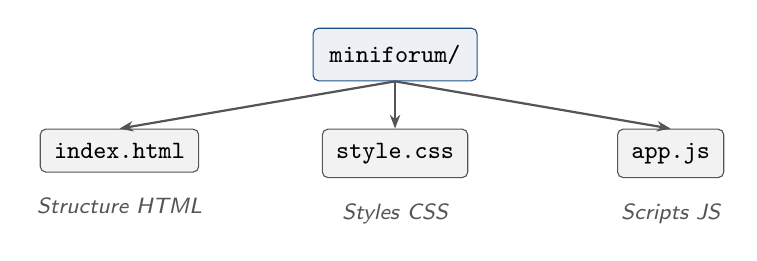
\begin{tikzpicture}[font=\small,
  folder/.style={draw=uniNavy, thin, rounded corners=2pt, fill=uniNavy!8,
    inner sep=6pt, font=\small\bfseries},
  file/.style={draw=uniGrey, thin, rounded corners=2pt, fill=uniPaper,
    inner sep=5pt},
  arr/.style={-{Stealth[length=5pt]}, uniGrey, thick}]

\node[folder] (root) {\texttt{miniforum/}};
\node[file, below=0.6cm of root, xshift=-3.5cm] (html) {\texttt{index.html}};
\node[file, below=0.6cm of root, xshift=0cm]    (css)  {\texttt{style.css}};
\node[file, below=0.6cm of root, xshift=3.5cm]  (js)   {\texttt{app.js}};

\draw[arr] (root.south) -- (html.north);
\draw[arr] (root.south) -- (css.north);
\draw[arr] (root.south) -- (js.north);

\node[below=0.2cm of html, font=\footnotesize\itshape, text=uniGrey]
  {Structure HTML};
\node[below=0.2cm of css, font=\footnotesize\itshape, text=uniGrey]
  {Styles CSS};
\node[below=0.2cm of js, font=\footnotesize\itshape, text=uniGrey]
  {Scripts JS};
\end{tikzpicture}
\end{center}

\newpage

% ============================================================
\section{Git --- Premiers pas}
% ============================================================

Git est un outil de \textbf{gestion de version} : il enregistre l'historique de chaque modification de ton code, permet de revenir en arrière en cas d'erreur, et facilite le travail en équipe. C'est un outil professionnel incontournable, utilisé dans tous les projets informatiques.

\subsection{Pourquoi utiliser Git ?}

Imagine que tu travailles sur ton projet MiniForum. Sans Git, tu te retrouves rapidement dans cette situation :

\begin{center}
\renewcommand{\arraystretch}{1.0}
\begin{tabularx}{\linewidth}{p{4cm}X}
  \toprule
  \rowcolor{uniNavy}
  \color{white}\textbf{Fichier} & \color{white}\textbf{Ce que tu essaies de faire} \\
  \midrule
  \rowcolor{uniPaper}
  \texttt{index.html} & Version qui marche \\
  \texttt{index\_final.html} & Tentative d'amélioration \\
  \rowcolor{uniPaper}
  \texttt{index\_final2.html} & Autre tentative \\
  \texttt{index\_VRAI\_final.html} & On ne sait plus\ldots \\
  \bottomrule
\end{tabularx}
\end{center}

\vspace{6pt}
Git résout ce problème : un seul fichier, un historique complet, la possibilité de revenir à n'importe quel état passé.

\begin{tcolorbox}[definition, title={Ce que Git permet de faire}]
\begin{itemize}
  \item \textbf{Sauvegarder} l'historique complet de son projet, modification par modification
  \item \textbf{Revenir en arrière} à n'importe quel état antérieur du code
  \item \textbf{Travailler en équipe} sans écraser le travail des autres
  \item \textbf{Expérimenter} sans risque, sur une branche séparée
  \item \textbf{Synchroniser} son travail entre plusieurs machines via GitHub
\end{itemize}
\end{tcolorbox}

\subsection{Les quatre zones de Git}

Git organise le travail en quatre zones distinctes. Comprendre ces zones est essentiel pour ne pas être perdu face aux commandes.

\vspace{8pt}
\begin{center}
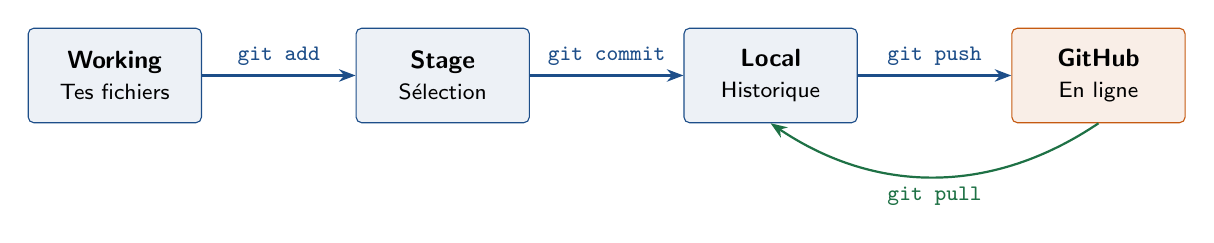
\begin{tikzpicture}[font=\small, node distance=1.95cm,
  state/.style={draw=uniNavy, thin, rounded corners=2pt, fill=uniNavy!8,
    minimum width=2.2cm, minimum height=1.2cm, align=center},
  remote/.style={draw=uniGold, thin, rounded corners=2pt, fill=uniGold!10,
    minimum width=2.2cm, minimum height=1.2cm, align=center},
  arr/.style={-{Stealth[length=6pt]}, thick}]

\node[state]  (wd)  {\textbf{Working}\\{\footnotesize Tes fichiers}};
\node[state, right=of wd]  (st) {\textbf{Stage}\\{\footnotesize Sélection}};
\node[state, right=of st]  (lo) {\textbf{Local}\\{\footnotesize Historique}};
\node[remote, right=of lo] (gh) {\textbf{GitHub}\\{\footnotesize En ligne}};

\draw[arr, uniNavy]
  (wd) -- node[above, font=\footnotesize]{\texttt{git add}} (st);
\draw[arr, uniNavy]
  (st) -- node[above, font=\footnotesize]{\texttt{git commit}} (lo);
\draw[arr, uniNavy]
  (lo) -- node[above, font=\footnotesize]{\texttt{git push}} (gh);

\draw[arr, uniTeal, bend right=-34]
  (gh.south) to node[below, font=\footnotesize]{\texttt{git pull}} (lo.south);

\end{tikzpicture}
\end{center}
\vspace{6pt}

\begin{center}
\renewcommand{\arraystretch}{1.0}
\begin{tabularx}{\linewidth}{p{4cm}X}
  \toprule
  \rowcolor{uniNavy}
  \color{white}\textbf{Zone} & \color{white}\textbf{Description} \\
  \midrule
  \rowcolor{uniPaper}
  \textbf{Working Directory} & Tes fichiers tels que tu les vois dans ton éditeur. Toutes tes modifications vivent ici. \\
  \textbf{Stage (Index)} & Zone de préparation : tu sélectionnes les fichiers que tu veux inclure dans le prochain commit. \\
  \rowcolor{uniPaper}
  \textbf{Repository local} & L'historique Git stocké sur ta machine. Chaque commit est un instantané du projet. \\
  \textbf{Remote (GitHub)} & Copie du dépôt hébergée en ligne. Permet la sauvegarde et le partage. \\
  \bottomrule
\end{tabularx}
\end{center}

\begin{tcolorbox}[astuce, title={Analogie --- La photo de groupe}]
Imagine que tu prépares une photo de groupe.
\textbf{Working Directory} : tout le monde est dans la salle.
\textbf{Stage} : tu demandes à certaines personnes de se mettre en position.
\textbf{Commit} : tu prends la photo --- c'est un instantané permanent.
\textbf{Push} : tu envoies la photo sur un serveur partagé pour que tout le monde y accède.
\end{tcolorbox}

\subsection{Commandes essentielles}

\begin{lstlisting}[language=bash, caption={Initialiser un projet Git}]
# Initialiser un depot Git dans le dossier courant
git init

# Voir l'etat des fichiers (modifies, en attente, non suivis)
git status

# Ajouter tous les fichiers modifies au stage
git add .

# Ajouter un seul fichier specifique
git add index.html

# Enregistrer un commit avec un message
git commit -m "Premier commit : structure de base du MiniForum"

# Voir l'historique des commits
git log --oneline
\end{lstlisting}

\begin{lstlisting}[language=bash, caption={Synchroniser avec GitHub}]
# Lier le depot local a un depot GitHub
git remote add origin https://github.com/votre-login/miniforum.git

# Envoyer les commits sur GitHub (premiere fois)
git push -u origin main

# Envoyer les commits suivants
git push

# Recuperer les modifications depuis GitHub
git pull
\end{lstlisting}

\begin{lstlisting}[language=bash, caption={Revenir en arriere}]
# Voir quelles modifications ont ete faites sur un fichier
git diff index.html

# Annuler les modifications d'un fichier (avant git add)
git restore index.html

# Voir le detail d'un commit
git show abc1234
\end{lstlisting}

\begin{tcolorbox}[astuce, title={Bonne pratique --- Messages de commit}]
Un bon message de commit décrit \textbf{ce qui a changé}, pas comment.\\[4pt]
\textcolor{uniTeal}{\textbf{OK}}\quad \texttt{Ajout formulaire création de sujet}\\
\textcolor{uniTeal}{\textbf{OK}}\quad \texttt{Correction bug affichage liste des messages}\\
\textcolor{BrickRed}{\textbf{NON}}\quad \texttt{modif} \qquad
\textcolor{BrickRed}{\textbf{NON}}\quad \texttt{ca marche} \qquad
\textcolor{BrickRed}{\textbf{NON}}\quad \texttt{update}
\end{tcolorbox}

\subsection{Le fichier \texttt{.gitignore}}

Certains fichiers ne doivent jamais être versionnés : mots de passe, dépendances téléchargées, fichiers temporaires. Le fichier \texttt{.gitignore} indique à Git quels fichiers ignorer.

\begin{lstlisting}[language=bash, caption={.gitignore --- Exemple pour MiniForum}]
# Dependances Node.js (a ne jamais committer)
node_modules/

# Variables d'environnement (mots de passe, cles API)
.env

# Fichiers systeme macOS
.DS_Store

# Fichiers temporaires de l'editeur
.vscode/settings.json
\end{lstlisting}

\begin{tcolorbox}[attention, title={Important --- Ne jamais committer \texttt{node\_modules/}}]
Le dossier \texttt{node\_modules/} peut contenir des milliers de fichiers et peser plusieurs centaines de mégaoctets. Il doit \textbf{toujours} figurer dans \texttt{.gitignore} : les dépendances se réinstallent en une commande (\texttt{npm install}), elles n'ont pas leur place dans l'historique Git.
\end{tcolorbox}

% ============================================================
\section{Lexique de la semaine}
% ============================================================

\begin{center}
\renewcommand{\arraystretch}{1.0}
\begin{tabularx}{\linewidth}{p{4cm}X}
  \toprule
  \rowcolor{uniNavy}
  \color{white}\textbf{Terme} & \color{white}\textbf{Définition} \\
  \midrule
  \rowcolor{uniPaper}
  URL & Adresse permettant de localiser une ressource sur le web \\
  DNS & Service qui traduit un nom de domaine en adresse IP \\
  \rowcolor{uniPaper}
  HTTP / HTTPS & Protocole de communication entre client et serveur (HTTPS = version chiffrée) \\
  Client & Programme qui demande une ressource (le navigateur) \\
  \rowcolor{uniPaper}
  Serveur & Programme qui répond à une demande en fournissant fichiers ou données \\
  Statique & Contenu identique quel que soit le visiteur ou le moment \\
  \rowcolor{uniPaper}
  Dynamique & Contenu généré à la demande, souvent depuis une base de données \\
  Commit & Enregistrement d'un instantané des modifications dans Git \\
  \rowcolor{uniPaper}
  Dépôt (repository) & Dossier suivi par Git, contenant l'historique du projet \\
  \bottomrule
\end{tabularx}
\end{center}

% ============================================================
\section*{Pour aller plus loin}
% ============================================================

\begin{tcolorbox}[astuce, title={Quiz et travaux pratiques}]
\begin{itemize}
  \item Un \textbf{quiz d'auto-évaluation} sur cette semaine est disponible sur Moodle.
  \item La \textbf{fiche TP} (mise en place de l'environnement et premier dépôt Git) est distribuée séparément : \textit{S01\_TP.pdf}.
\end{itemize}
\end{tcolorbox}

% ============================================================
\section*{Résumé de la semaine}
% ============================================================

\begin{tcolorbox}[definition, title={Ce qu'il faut retenir}]
\begin{itemize}
  \item Le web fonctionne sur un modèle \textbf{client / serveur} via le protocole \textbf{HTTP}
  \item Le \textbf{DNS} traduit un nom de domaine en adresse IP
  \item \textbf{HTML} structure, \textbf{CSS} présente, \textbf{JavaScript} rend interactif
  \item Un site \textbf{statique} renvoie toujours le même contenu, un site \textbf{dynamique} le génère à la demande
  \item \textbf{Git} : \texttt{add} $\to$ \texttt{commit} $\to$ \texttt{push} pour versionner son code
  \item \textbf{MiniForum} sera le projet fil rouge développé progressivement sur 15 semaines
\end{itemize}
\end{tcolorbox}

\vspace{8pt}
\begin{tcolorbox}[attention, title={Pour la semaine 2}]
\begin{itemize}
  \item Vérifier que VS Code, Node.js et Git sont correctement installés
  \item Créer son compte GitHub si ce n'est pas déjà fait
  \item Avoir son dépôt \texttt{miniforum/} initialisé avec les trois fichiers de base et poussé sur GitHub
\end{itemize}
\end{tcolorbox}

\end{document}
